%!TEX encoding = UTF8
%!TEX root = 0-notes.tex

\chapter{Suites}

\section{Introduction}

\dfn{suite}{
	On appelle \emph{suite} une fonction $u$ réelle prenant des entiers naturels $n\in\N$.
	
	Le \emph{terme initial} de la suite est donné par $u(0)$.
	Le \emph{terme de rang $n$} de la suite est donné par $u(n)$.
}{dfn:suite}

\nt{
	Une suite est une liste de valeurs réelles $u(0), u(1), u(2), \dots$.
	On peut connaitre tous les termes d'une suite dès qu'elle est définie \emph{algébriquement}.
	C'est-à-dire, si $u(n) = \big(\text{expression en fonction de $n$}\big)$ pour tout $n\in\N$.
}

\ex{}{
	La suite donnée algébriquement par $u(n) = n-1$ pour tout $n\in\N$ est entièrement connue.
	Son terme initial est $u(0) = -1$, et son terme de rang $210$ est $u(210) = 209$.
}{ex:suite-alg}

\ex{}{
	Les fonctions suivantes sont des suites données par leur rang $n$ : on connait donc leur valeur pour tout les entiers naturels.
	\begin{multicols}{2}
	\begin{enumerate}
		\item $u(n) = n+1$
		\item $v(n) = n^2$
		\item $\xi(n) = \dfrac1{n^3}$
		\item $a(n) = (n+1)^n$
	\end{enumerate}
	\end{multicols}
	Une suite n'a pas forcément de formule générale pour tout $n$, c'est une simplement \emph{suite} de nombres réels.
}{}

\nt{
	Certaines suites peuvent être définies \emph{récursivement}.
	Le terme de rang $n$ dépendra des termes de rangs inférieurs.
}

\ex{}{
	Considérons la suite $u$ de terme initial $u(0) = 0$ et vérifiant, pour tout $n\in\N$,
		\[ u(n+1) = u(n) + 2. \]
	On lit « le terme de rang $n+1$ est égal au terme de rang $n$ plus 2 » ou, autrement dit, « pour passer d'un terme au suivant, il faut ajouter 2 ».
	Ainsi $u(1) = u(0) + 2 = 2, u(2) = 4, u(3) = 6, \dots$.
	
	Pour calculer $u(341)$, il faut, \emph{a priori} nécessairement calculer tous les termes de rang inférieur à $341$.
	Cependant, il semblerait $u(n) = 2n$ pour tout $n\in\N$, et donc qu'on ait immédiatement $u(341) = 682$.
}{ex:suite-rec}


\section{Implémentation}

\exe{}{
	On appelle $H_n = \sum\limits_{k=1}^n \dfrac1k$ la \emph{série harmonique}.
	Implémenter la fonction $H_n$ et donner la valeur approximative de $H_{100}$.
	Ensuite, trouver le premier rang $n$ vérifiant $H_n \geq 10$.
}{exe:serie-harmonique}{
	Voici deux implémentation de $H_n$ possibles. On obtient $H_{100} \approx 5,1873$.

	\begin{multicols}{2}
	\python{harmonic-series}
	\columnbreak
	\python{harmonic-series-2}
	\end{multicols}
}

\exe{}{
	Trouver le premier rang $n$ vérifiant $H_n \geq 10$, où $H_n$ désigne la série harmonique définie à l'exercice \ref{exe:serie-harmonique}.
}{exe:seuil-harmonique}{
	Voici une implémentation permettant de trouver le premier rang $n$ vérifiant $H_n \geq 10$. On obtient $n=12369$.
	
	\python{harmonic-series-3}
}



\exe{}{
	Implémenter l'algorithme \ref{alg:seul-geom} et trouver le plus petit entier naturel $n\in\N$ vérifiant les inéquations suivantes.
	\begin{multicols}{2}
	\begin{enumerate}
		\item $2 \times 3^n > 100~000$
		\item $7 \times \left(\dfrac32 \right)^n > 50~000$
		\item $3 \times \left( \dfrac43 \right)^n > 1~000$
		\item $3 \times \left( \dfrac43 \right)^n > 10~000$
	\end{enumerate}
	\end{multicols}
}{exe:seuil-geom}{
	TODO
}

\section{Sommes}

\exe{,difficulty=1}{
	On considère la série statistique $X=(0;1;2;\dots;19;20)$.
	Justifier sans calcul que la moyenne de $X$ est $10$.
	En déduire que $1+2+\cdots+19+20 = 210$.
}{exe:moyenne}{
	Par symétrie autour de $10$, la moyenne de $X$ vaut $10$ : toute valeur $10+k$ se compense avec $10-k$ pour $k=1, \dots, 10$, et la valeur $10$ seule est moyenne et n'a donc aucun impact.
	
	La formule de la moyenne donne $\dfrac{1+2+\cdots+19+20}{21} = 10$, d'où le résultat.
}

\thm{}{
	Pour tout $n\in\N$, on a l'égalité	
		\[ 0 + 1 + 2 + \cdots + n = \dfrac{n(n+1)}2. \]
}{thm:triangle}

\pf{}{
	Posons $S_n = 1 + 2 + \cdots + n$ pour $n\in\N$.
	
	\begin{multicols}{2}
	On considère le carré $(n+1) \times (n+1)$ ci-contre, découpé en $(n+1)^2$ carrés unités.
	
	En comptant les carrés sur chaque diagonale, on a 
		\[ S_n + (n+1) + S_n = (n+1)^2,\]
	ce qui conclut.
	
	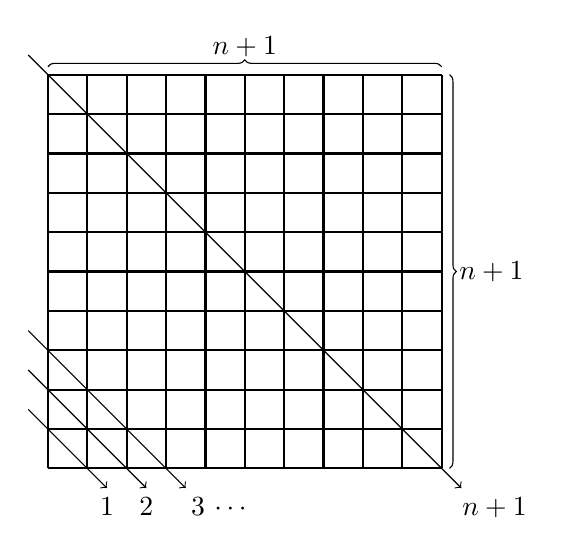
\begin{tikzpicture}[scale=0.5]
		\foreach \r in {0, ..., 10} {
			\draw[black,thick] (0,\r) -- (10,\r);
			\draw[black, thick] (\r,0) -- (\r, 10);
		}
		
		\draw[decoration={brace},decorate]
  			(0,10.2) -- node[above] {$n+1$} (10,10.2);
		\draw[decoration={brace, mirror},decorate]
  			(10.2,0) -- node[right] {$n+1$} (10.2,10);
  			
		\draw[->] (-0.5, 1.5) -- (1.5,-0.5) node[below] {$1$};
		\draw[->] (-0.5, 2.5) -- (2.5,-.5) node[below] {$2$};
		\draw[->] (-0.5, 3.5) -- (3.5,-.5) node[right=12pt, below] {$3$ $\cdots$};
		
		\draw[->] (-0.5, 10.5) -- (10.5,-.5) node[right=12pt, below] {$n+1$};
	
	\end{tikzpicture}
	\end{multicols}
}

\nomen{
	On appelle $S_n$ un \emph{nombre triangulaire} car il apparaît comme le nombre de carrés dans le triangle de la preuve du théorème \ref{thm:triangle}.
}

\notations{
	Au lieu de noter $S_n = 1 + 2 + \cdots + n$, on dit à l'oral « la somme des entiers de 1 à $n$ », car c'est plus court.
	On dit aussi « la somme des $k$, $k$ allant de 1 à $n$ », qu'on choisit de noter
		\[ S_n = 1 + 2 + \cdots + n = \text{« la somme des $k$, $k$ allant de 1 à $n$ »} = \sum_{k=1}^n k, \]
	où la lettre sigma majuscule $\Sigma$ désigne une somme.
	
	Plus généralement, on note
		\[ \sum_{k=a}^b u(k) = u(a) + u(a+1) + \cdots + u(b-1) + u(b). \]
}

\nt{
	Il est également possible d'indexer une somme sur un ensemble.
	Par exemple pour $E=\bigset{7; 11; 13 ; 17}$, 
		\begin{align*}
			\sum_{k\in E} k = 7+11+13+17 = 48, && \text{ et } && \sum_{k\in E} \dfrac1k = \dfrac17+\dfrac1{11}+\dfrac1{13}+\dfrac1{17} \approx 0,3695.
		\end{align*}
	
	Le deuxième théorème de Mertens implique que
		\[ \sum_{p \text{ premier}} \dfrac1p = \pinfty. \]
}

\exe{}{
	Donner les valeurs des sommes suivantes.
	\begin{multicols}{3}
		\begin{enumerate}[label=\roman*)]
		\item
		$\sum\limits_{k=1}^{10} 0$
		
		\item
		$\sum\limits_{k=1}^{10} 1$
		
		\item
		$\sum\limits_{k=0}^{10} 1$
		
		\item
		$\sum\limits_{k=-5}^{11} 1$
		
		\item
		$\sum\limits_{k=4}^{8} 2$
		
		\item
		$\sum\limits_{k=0}^{n} 1$
		
		\item
		$\sum\limits_{k=1}^{10} k$
		
		\item
		$\sum\limits_{k=1}^{20} k$
		
		\item
		$\sum\limits_{k=11}^{20} k$
		\end{enumerate}
	\end{multicols}
}{exe:sommes}{
	\begin{multicols}{3}
		\begin{enumerate}[label=\roman*)]
		\item
		$\sum\limits_{k=1}^{10} 0 = 0$.
		
		\item
		$\sum\limits_{k=1}^{10} 1 = 10$.
		
		\item
		$\sum\limits_{k=0}^{10} 1 = 11$.
		
		\item
		$\sum\limits_{k=-5}^{11} 1 = (11 + 5 + 1) = 17$.
		
		\item
		$\sum\limits_{k=4}^{8} 2 = 2(8-4+1) = 10$.
		
		\item
		$\sum\limits_{k=0}^{n} 1 = n$.
		
		\item
		$\sum\limits_{k=1}^{10} k = \dfrac{10(11)}2 = 55$.
		
		\item
		$\sum\limits_{k=1}^{20} k = \dfrac{20(21)}2 = 210$.
		
		\item
		$\sum\limits_{k=11}^{20} k = \sum\limits_{k=1}^{20} k - \sum\limits_{k=1}^{10} k = 210-55 = 155$.
		\end{enumerate}
	\end{multicols}
}

\thm{linéarité de la somme}{
	Pour $c\in\R$ et $u, v,$ deux suites, on a 
		\[ \sum_{k=a}^{b} \bigl[ cu(k) + v(k) \bigr] =  c\sum_{k=a}^{b} u(k)+ \sum_{k=a}^{b}v(k). \]
}{thm:linéarité-somme}

\exe{,difficulty=1}{
	Démontrer le théorème \ref{thm:linéarité-somme}.
}{exe:linéarité-somme}{
	En explicitant la somme
		\[ \sum_{k=a}^{b} \bigl[ cu(k) + v(k) \bigr] = cu(a) + v(a) + cu(a+1) + v(a+1) + \cdots + cu(b) + v(b), \]
	on remarque qu'on peut regrouper les termes et factoriser par $c$ pour obtenir
		\[ \sum_{k=a}^{b} \bigl( cu(k) + v(k) \bigr) = c\bigl[u(a) + u(a+1) + \cdots + u(b)\bigr] + \bigl[v(a) + v(a+1) + \cdots + v(b)\bigr] = c\sum_{k=a}^{b} u(k)+ \sum_{k=a}^{b}v(k). \]
}
